\graphicspath{{chapters/4.Chapter_2/figures}}

\begin{savequote}[75mm]
"even after the observation of the frequent or constant conjunction of objects, we have no reason to draw any inference concerning any object beyond those of which we have had experience;"
\qauthor{- David Hume: \textit{A Treastie of Human Nature, 1738}}
\end{savequote}


\chapter{Transcriptomic analysis of the \textit{Paramecium bursaria} and \textit{Micractinium reisseri} endosymbiosis}

\section{Introduction}

Transcriptomics, and specifically RNA-Seq, is a powerful method by which the \textit{Paramecium bursaria}-\textit{Micractinium reisseri}
endosymbiosis can be investigated. This endosymbiosis conveys phototrophy \citep{Karakashian1963} as well as 
numerous photobiological behavioural and biochemical traits (e.g. \citep{Berk1991,Saji1974,Nakajima1989,Niess1982a,Iwatsuki1988,Summerer2009}, 
partially reviewed in \citep{Sommaruga2009}).  Additionally, photosynthesis and unidentified light-induced factors have been identified as key to the establishment
and maintenance of this endosymbiosis (and prevention of algal digestion by the host) \citep{Karakashian1963,Hosoya1995a,Kodama2007,Kodama2014c}.
Therefore, a (relatively) unbiased global metatranscriptomic profile of host and endosymbiont in both lit and dark conditions can be used to 
identify key transcripts playing a role in the establishment, maintenance, and photobiological traits of this endosymbiosis. 
%constitutively expressed photosynthetic components
This profile will allow metabolic reconstruction of host and endosymbiont in both photosynthetically active and inactive
states as well as offering a means to identify significantly differentially expressed transcripts between these states.


The effectiveness of this approach is evidenced by several studies (e.g. \citep{Nowack2011,Jiggins2013,Xiang2015}) investigating
host-chloroplast interactions. Such transcriptomic methods, focussing on a limited and defined number of interacting organisms, and thus falling 
falling between analysis of axenic cultures and
large scale metatranscriptomics, have been dubbed by some ``dual-RNAseq'' \citep{Westermann2012}.  
``Dual-RNASeq'' methods are exemplified by Tierney \textit{et. al.} in the context of eukaryote-eukaryote host-pathogen interactions \citep{Tieryney2012}.


The plethora of literature relating to the physiology and behaviour of \textit{Paramecium bursaria} and green algal endosymbioses (e.g. \citep{Iwatsuki1988}, 
    see \citep{Kato2009a} and \chap{introduction} for more details) as well as the relative transcriptomic tractability demonstrated separately in relatives of
    both of these organisms (e.g. \citep{Guarnieri2011,Rowe2014,Bashan2015} and \citep{Arnaiz2010,Kolisko2014})\footnote{It may be worth noting
        that \citep{Guarnieri2011} is an example of \textit{C. vulgaris} transcriptome without a reference genome, and \citep{Kolisko2014} undertook
    a preliminary single cell transcriptomic approach to analysing a species of \textit{Paramecia}}
and together \citep{Kodama2014} makes \textit{Paramecium bursaria} - \textit{Micractinium reisseri} (PbMr)
well suited for such a ``dual-RNAseq'' analysis.  

Having said this, dual-RNAseq in the PbMr system also presents difficulties which must be overcome to facilitate effective analysis.
Principally, accurately reconstructing transcripts from a complex, relatively genomically uncharacterised, system and 
that of subsetting these transcripts into groups dependent on their originating organism.  This latter step is particularly important
as it allows the removal of transcripts originating from bacterial food species of the mixotrophic host, as well as from other potential
host endosymbionts and general sequencing contamination.  


Towards this end we conducted a bulk RNA-Seq sequencing of cultured PbMr using 76bp paired-end reads and the Illumina GAII platform.
Unfortunately, due to limitations in the maintainable culture density of the \textit{Paramecium bursaria} CCAP 1660/12 and thus the quantity of extractable
mRNA it was necessary to pool all day and night replicates into a single pair of day and night libraries. 
While this provided sufficient material for sequencing it precluded accurate inference of significant differential expression between day or night
as it masked all biological replicates \citep{Auer2010}.  We, therefore, also sequenced a set of 3 (followed later by an additional 5) dark and 3 light
biological replicates using single-cell RNA-Seq (scRNA-Seq) methods. 


scRNA-Seq is a relatively new set of technologies facilitating sequencing transcriptomes from miniscule quantities of starting material, on the order of picograms
and from 1 to a few cells (reviewed \citep{Macaulay2014,Liang2014,Wu2014a}).  Specifically, we used a poly-A reverse-transcription
and multiple displacement amplification (MDA) based method.  
This was chosen instead of other scRNA-Seq methods e.g. Quartzseq \citep{Sasagawa2013} or 
Tang's method \citep{Tang2009} as its base method (MDA) has been widely applied and characterised in single cell genomics (i.e. \citep{Spits2006}) and is
relatively WHY?


It is also among the cheaper, simpler and easily available scRNA-Seq kits 
%SMARTSEQ is 1.3k for 12rxns maybe checkw ith david



While nascent, these technologies have shown a lot of promise in well characterised systems such as human cell cultures \citep{Bengtsson2005,Shalek2013}
and \textit{Saccharomyces cerevisiae} \citep{Lipson2009}.  
    Additionally, there are high expectations of them as emerging technologies to address difficult outstanding issues in ``dual-RNASeq'' \citep{Westermann2012} and transcriptomics 
    in general.
Specifically, allowing analysis of unculturable or poorly culturable systems \citep{Murray2012} and offering a means to investigate cell-cell heterogeneity 
in expression patterns (e.g. \citep{Raj2008,Shalek2013}).  This is important as it reduces the risk of a Yule-Simpson effect \citep{Yule1903a,Simpson1951}, where
distinct expression patterns in subpopulations of cells could generate a spurious overall pattern if falsely amalgamated (as may occur in population level
bulk RNA-Seq).  However, as best as I can tell there has only been one published use of scRNA-Seq in non-model unicellular eukaryotes without genomic resources.
This study by \citet{Kolisko2014} briefly addressed bias, contamination and gene discovery effectiveness in a set of complex unicellular eukaryotic
systems.  However, it used a SMART based approach instead of MDA \citep{Kolisko2014} and didn't address in depth the optimal way to process, assemble and utilise
single cell datasets.


These samples present an opportunity to investigate in-depth the most effective way to use MDA-based scRNA-Seq in a complex
eukaryotic ``dual-RNASeq'' system as well the general feasability of such an approach.  For example, is the best use of this sort of data to use
bulk and SCTs together for assembly, or is it more efficient to use a bulk assembly as a reference and map the single cell reads to it for quantification
and/or further assembly (i.e. referenced assembly of SCT data subset which maps to bulk transcriptome, and then further \textit{de novo} assembly
of remaining transcripts)?


%However, MDA is prone to a degree of amplification bias \citep{Liang2014} which may be problematic in accurate inference of differential expression
%therefore, the suitability of MDA-based scRNA-Seq in particular will also need to be assessed.

%The only other published analysis of \textit{Paramecium bursaria} and its green algal endosymbionts by \citep{Kodama2014} largely
%side-stepped this issue by focussing on the analysis of host transcripts with and without the endosymbiont by filtering
%likely endosymbiont derived contigs from analysis using a crude MEGABLAST \(e^{-40}\) approach.
%Studies in related ciliates have demonstrated a high prevalence of alternative splicing events (5.2\% of genes in \textit{Tetrahymena
%    thermophila} for a single celled eukaryote \citep{Xiong2012}
%This paper also demonstrated the huge dynamic range of expression (and thus necessity of RNA-Seq over microarray approaches) in \textit{T. thermophila})
%with approximately 6 order of magnitude range \citep{Xiong2012}

%However, as both target species - host and endosymbiont are eukaryotes the complication of mRNA enrichment 
%is simplified due to the sufficiency of poly-A selection for this task (instead of rRNA depletion methods)
%Determining the necessary sequencing depth is also difficult.

%One advantage of the single cell approach is that due to the ligation step prior to WTA
%terminal coverage issue of bulk RNA-Seq should be mininised.  This is particularly important as it is
%expected that secreted peptides are likely to play an important role in maintenance of any cellular relationship
%that involves multiple intermediate membranes and secretion is frequently controlled by terminal peptide sequences.

%First achieved in \citep{Lao2009}


Therefore, this chapter addresses the key difficulties of accurately recapitulating transcripts from the \textit{Paramecium bursaria}
and \textit{Micractinium reisseri} system \textit{de novo} as well as 
determining the optimal way in which 2nd generation bulk and single cell RNAseq libaries may be integrated together in a complex 
reference-free system.
Specifically, we seek to generate methods by which libraries may be screened before assembly, 
determine the optimal preprocessing (trimming and error correction), optimal assembler and \textit{de novo} 
assembly parameters, the utility of very divergent related genomes as a ``reference'', and/or mixed
self-mapping assembly methods between bulk and SCT data. 
Finally, developing a means of accurate transcript binning into putative species origins.


\subsection{Assembly}

Much as library contamination is one of the key issues with single cell genomics \citep{Blainey2013,Lusk2014}, it is a key
issue in single cell transcriptomics.  Single cell methods are particularly prone to contamination issues
from reagents, laboratory environment and enigmatic nucleic acids within the biological samples themselves due to 
low-input concentration and high amplification necessary found in these approaches \citep{Blainey2013}.
Furthermore, when utilising single cell libraries in a \textit{de novo} assembly instead of merely mapping
it is doubly important to attempt to discard libraries that are likely to be contaminated by unwanted
reads.  The importance of this was observed during preliminary assemblies when the inclusion of particular
libraries were liable to fragment and hugely expanding the resultant assembly.  

Additionally, these methods


Therefore, to this end a set of scripts, known as ``dueydrop'', were developed to allow rapid taxonomic profiling of a
representative subset of each library.  These profiles can then be manually analysed or grouped using unsupervised learning methods 
to investigate the existence of outlier libraries likely to be the product of contamination or sequencing failure.
The user can then determine, based on heuristics of their dataset, which libraries are to be included in downstream analyses.
The utility of a tool capable of this form of rapid taxonomic screening of sequenced libraries is evidenced
by the emergence of commercial platforms providing such tools as a cloud service e.g. \url{http://blog.onecodex.com/}



While there has been some analysis of optimal trimming for bulk RNA-Seq (particularly \citep{MacManes2014})
there has not been an investigation of the optimal trimming parameters for single cell RNA-Seq Illumina reads.
Correct trimming is important to minimise sequence error (mostly substitutions \citep{Yang2013}) as these
result in assembly of spurious sequences \citep{Macmanes2013,MacManes2014}.  Therefore, to determine
optimal trimming parameters for the raw single-cell paired-end RNA-Seq reads 
a naive grid search algorithm using random reads sub-sampled from each library was used and effect on mapping
statistics against a ``baseline'' Trinity assembly of bulk reads \citep{Haas2013}.
Additionally, there has been emerging evidence that error correction is a key stage in the accurate
recapitulation of reads, especially from single cell libraries \citep{Medvedev2011}.  Therefore, the effect and feasability 
of read error correction on this assembly was also assessed.  
The efficacy of digital normalization, a method to remove redundant read data from libraries and thus
reduce the computational burden of assembly \citep{Brown2012}, was also investigated for this dataset.
Interestingly, some have argued that error correction is special case of general digital normalization
\citep{Krasileva2013}.


Finally, on the basis of the strong GC-AT bias exhibited by host and endosymbiont transcripts
the performance of pre-assembly read partitioning using a custom clustering tool known as
ParKour was assessed.  The logic behind this was based on the clear bimodal GC distribution
displayed in FastQC library quality checking as well as known 30\% host and 50\% endosymbiont
GC biases from sequenced genomes of relatives (i.e. \textit{P. tetaurelia} \citep{Aury2006} and 
\textit{Chlorella} NC64A \citep{Blanc2010a}) and the occasional practice of binning found in
meta-omic analyses (for example those discussed in \citep{Droge2012}).  Theoretically, accurate
pre-assembly read binning could transform a complex assembly graph into two relatively simpler
assembly tasks.  As well as simplifying path resolution accuracy, if this method were to work
it would speed up assembly considerably and thus allow more iterations to optimise other
assembly paramters.

As we expect the PbMr metatranscriptome to contain predominantly a highly AT-rich organism, \textit{Paramecium},
(ranging from 24.1 to 28.2\%GC in \textit{P. aurelia} species complex and \textit{P. caudatum} \citep{Aury2006,McGrath2014})
and a very GC-rich organism, \textit{Micractinium}, (\textit{Chlorella variabilis} NC64A genome is approximately 67.1\%GC, the highest
found in a sequenced eukaryote genome (in 2010) \citep{Blanc2010}).  



Although intriguingly low-GC regions 55-65\%GC have a significantly higher number of mapped genes suggesting they are highly expressed \citep{Blanc2010}

Also correlations with increased GC richness in highly expressed regions of paramecium

Therefore,  would be closer than whole genome richness but still separable, this can be seen in the bimodal GC distribution in the raw and trimmed sequencing 
reads.

\begin{figure}
    Example GC plot showing bimodal distribution
\end{figure}

Due to the difficulties generating a high quality \textit{de novo} metatranscriptome assembly, I considered  it worth investigating whether there could be GC\%
clusters and furthermore whether assigning reads to these clusters and assembling the reads corresponding to a cluster would generate any meaningful groupings of reads.

To this end, I 






Unfortunately, while it is possible to infer pre-processing parameterisation and options that
are likely to improve an assembly using heuristic measures like mapping metrics
it is very difficult to accurately say which paramaters 
will lead to the ``best'' assembly.  Assembly is an example of
Wolpert and Macready's ``No Free Lunch Theorems'' \citep{Wolpert1995,Wolpert1997} 
as \textit{de novo} as it is fundamentally a hamiltonian/eulerian cycle search problem (equivalent
    in the de-Bruijn formulation) and therefore any two assembly implementations (in different assemblers and/or
    with different parameters) should ultimately be equivalent across all possible input datasets.\footnote{
    This should be taken with a pinch of salt, a proof of this theorem applied to the case of assembly is beyond
both the scope of this thesis and my abilities}





Error correction of Illumina reads has been considered by some authors as a key
step in the assembly of error-correction.  This is particularly true for single-cell
data generated via MDA. 
Error-correction is typically achieved by discarding lowly expressed k-mers 
as these are likely to have been generated by errors.









With candidate optima identified for read/library pre-processing, assembly itself could be 
attempted.  Consequently, several assemblers and a range of assembly settings were 
used and compared to determine the ``best'' assembly.   Both \textit{de novo} assembly
in which transcripts were attempted to be recovered using just raw bulk and single cell
PE Illumina libraries and referenced assemblies were attempted.







The task of identifying the ``best'' \textit{de novo} transcriptome assembly is also a non-trivial 
task \citep{Neil2013}.  Many widely used assembly assessment metrics have been shown to be
inconsistent measures in simulated sequencing data, especially those metrics related to invidual
contigs (theoretically different transcript splices).  Metrics such as average length and N50
prove consistent across both simulated sequencing depth and read lengths i.e. they improve 
towards \citep{Neil2013}.  Furthermore, the number of possible metrics is greatly reduced
if assessment mainly is conducted in a reference-free manner (i.e. not based on comparison
to transcripts derived from other sequencing projects).   A reference-free approach was chosen
primarily 










due to the divergence
of related organisms in thi






Average unigene () length, \% of reads used in contigs, unigene N50






with many suggested methods and metrics.





\subsection{Binning}

However, even once a good assembly has been generated it is still necessary to identify the likely
originating species of a given transcript i.e. host, endosymbiont, food bacterial contaminant or other
contaminant.  While a successful partitioned assembly strategy may simplify this process it would still
be sensible to confirm bins using downstream analyses that use full length assembled transcripts and thus
more potential data than are present in shorter individual PE reads.  Rough, approximate bins were
generated using a simple "top BLAST hit" approach following ORF calling (using Tetrahymena and Universal
encodings) against a set of representative predicted proteomes.  In order to assess how accurate these
bins were likely to be, 10,000 were randomly selected and rapid maximimum-likelihood phylogenies were
generated using the transcript sequence as a seed to sample the entire RefSeq protein nr database.
This was accomplished using ``Dendrogenous'', a rewritten and modified version of a pipeline originally known 
as ``Darren's Orchard'' which first appeared in \citep{Richards2009g}.  Phylogenies were manually assessed to check
whether the resultant topology was congruent with the BLAST based binning i.e. are supposedly ``endosymbiont''
transcripts branching principally with archaeplastida taxa.  


While, due to the painfully manual nature of this phylogeny assessment process, 
it would be infeasible to repeat this phylogeny binning procedure for all transcripts, ``Dendrogenous'' allowed
relatively rapidy generation of phylogenies for all transcripts.  Therefore, this presented an ideal
challenge for supervised classification with the corpus of 10,000 manually validated phylogenies providing an effective
training dataset for a supervised classification algorithm.  









%%Can you separate transcripts from host, endosymbiont and food bacteria?
%Current practices and how they were applied - BLAST, GC etc
%Initial binning vs phylogenetics - seems better
%But still too work intensive - use manually done 10,000 for rest of transcriptome therefore ML
%Flowchart of tool 
%t-SNE plot of vectors
%classifier log-loss and learning curve comparison using logistic regression, SVM with diff kernels
%Convergence check for SVM hyperparameters
%anomaly detection?
%
%Transcriptome Assembly:
%
%- Trimming: MacManes 5, 30 (also did 12 and 35)
%- Error correction: Spades error correction
%- GC clustering parKour
\section{Methods} 

\subsection{Sample Preparation and Sequencing}

\subsubsection{Bulk transcriptomic RNA preparation}
For bulk transcriptomic analyses CCAP 1660/12 cells were harvested in a way to minimise the 
number of bacterial prey species from the culture, \textasciitilde \(10^{6}\) 
cell aliquots were strained through \(40\mu m\) sieves, filtered on 
\(10 \mu m\) nylon filters, 
before finally being filtered on \(8 \mu m\) TETP polycarbonate filters using a 
low-pressure filtration pump.  Collected samples were either immediately 
quick-frozen in liquid nitrogen for storage (\(-20\)\celsius for short-term storage 
and \(-80\)\celsius for longer storage) or harvested by centrifugation.  
In order to investigate the two main metabolic states of the symbiosis 
(i.e. under light conditions during active photosynthesis and in the dark 
when no photosynthesis is taking place) samples were extracted 5 hours into 
the light and dark phase of the 12:12 hour day-night cycle.

To ensure extracted RNA was representative of healthy and interacting host 
and endosymbionts care was taken to minimise the number of dead/dying cells 
from which RNA was extracted.  In order to do this, a subsample was taken 
from each culture during the process of harvesting and scored for dead/dying cells.  
Cell assays were formed by taking 1-2ml of each harvest cell pellet and 
fixed using 40\(\mu l\) Lugol's solution (0.5g \(I_{2}\) and 1g KCl in 8.5ml 
of MilliQ water). Dead/dying cells were identified as broken or puckered cells 
and counted using light microscopy.  Samples containing >10\% dead/dying cells 
were discarded and no RNA extracted from them.

In order to lyse collected samples, cells were washed from the filter or the 
pellet was resuspended in 1ml TriReagent (Sigma) heated to \(60\)\celsius. 
Cells were vortexed with sterile \(300\mu m\) glass-beads for 15s, incubated at 
room temperature for 10 minute, vortexed for 15s, quick-frozen in liquid 
nitrogen and stored at \(-20^{o}C\) before further processing.  
Samples were defrosted, vortexed for 15s, placed in a heat-block set 
to \(60^{o}C\) for 10 minutes while continuing to be vortexed, removed from 
heating and vortexed again for 15s.  
RNA was extracted by adding 0.2ml of Chloroform to the glass-bead-trizol-sample 
solution, shaking for 15s, incubating for 5 minutes at room temperature and 
centrifuging at 12,000g for 15 minutes at $4^{o}$C.  
The upper-phase was then transferred to an RNAse-free 1.5ml tube and an 
equal volume (\textasciitilde$0.5$ml) of isopropanol was added before shaking for 15s.  
The isolated RNA was then incubated at $-20^{o}$C for 10 minutes 
(up to several hours) before being collected as a pellet using a centrifuge at 
10,000g for 10 minutes at $4^{o}$C (supernatant was discarded). 
The RNA pellet was then washed with 1ml of 75\% ethanol and centrifuged 
twice at 10,000g for 10 minutes at $4^{o}$C with the supernatant being 
discarded after each centrifugation.  
Pellet was dried before being resuspended in 100$\mu l$ of RNAse-free water.  
The RNA was then cleaned further using the Qiagen RNeasy clean-up kit 
before being assessed for quality using ND-1000 (NanoDrop) and BioAnalyzer (Agilent).


\subsubsection{Single Cell RNA preparation}

For single cell transcriptomics, a ``cell-picking'' approach was used in which
\textit{P. bursaria} cells (from the CCAP1660/12 culture) were inspected on an inverted light microscope 
before being picked using an orally aspirated drawn-glass Pasteur pipette \citep{Garcia-Cuetos2012}.
In order to mininmise contamination from food bacteria present in the media these picked cells
were washed 3 times by serial transfer to \(10\mu l\) droplets of sterile NCL media.
The washed cell was then transferred to a \(10\mu l\) droplet of sterile water.
3 cells were picked 5 hours into both the lit and dark phase of the 12:12 hour day-night cycle.

Cells were transferred from their respective \(10\mu l\) droplets of sterile water to
a PCR tube containing \(6\mu l\) water and \(4\mu l \) lysis buffer (from the Qiagen
REPLI-g WTA Single Cell Kit) \citep{Korfhage2015}. To disrupt the cell beads (Sigma, \(425-600\mu m\), acid-washed)
were added to the meniscus, before submersion in liquid nitrogen for 5 seconds.  The sample was 
then thawed before vortexing for 1 minute.  
mRNA was selectively amplified and reverse transcribed to cDNA using poly-A selection.  The cDNA
was then amplified using multiple displacement amplification and the amplified cDNA purified
using a QIAamp DNA mini kit eluted in \(100\mu l\) elution buffer.

Subsequently, this process was repeated for a further 5 dark samples.

%\subsubsection{Single Cell genomic DNA preparation}
%Cells were transferred from their respective \(10\mu l\) droplets of sterile water to a microncentrifuge tube.
%CTAB method adapted from \citep{Winnepenninckx1993}.  Cells were disrupted by vortexing for 5 minutes with
%\(748.5\mu l\) CTAB extraction buffer (at 37\celsius) and ceramic beads (Sigma, \(425-600\mu m\), acid-washed).
%The tube was then incubated for 50 minutes at 37\celsius, vortexed for 5 minutes, and incubated for a further 50
%minutes at 60\celsius. DNA was extracted 3 times using phenol, chloroform and isoamylalcohol at a 25:24:1 ratio (pH 8),
%washed with 70\% ethanol and re-suspended in \(2.5\mu l\) TE buffer (pH 8). This DNA then underwent 
%Multiple displacement-based whole genome amplification using the Repli-G Single Cell Kit before purification using a 
%QIAmp DNA mini kit before elution in \(100\mu l\) elution buffer.  

\subsubsection{Library preparation}

For both bulk and single cell preparations each cDNA sample was fragmented in \(130\mu l\) 1xTE buffer on the Covaris E220 
with a target size of \(225bp\) (duty factor of \(10\%\), 200 cycles per burst, peak incident power
of 175, \(200s\) at \(7^{o}C\)). Fragment sizes were checked on a BioAnalyzer (Agilent) 7500 DNA chip.
cDNA was then concentrated using a GeneRead kit column with a elution in \(35\mu l\). Fragmentation
step was then repeated 3 times (\(110s\)) until majority of cDNA in each library was between \(200-250bp\)

cDNA ends were then end-repaired, adenylated and adapters ligated using the NEXTFlex (Biooscientfic) sequencing kit 
according to the manufacturer's instructions and using NEBNext (New England Biolabs) indices.  Also following
the NEXTFlex kit instructions, MgNa bead purification was done before and after PCR amplification using
NEBNext reagents.  Finally, prepared libraries were size selected using a Blue Pippin machine at a size selection
of \(350bp\) (range \(315-385bp\)).

A final bioanalyzer step was conducted with individual library concentrations ranging from \(0.66-4.09nM\).

\subsubsection{Sequencing}

The bulk day and night library were paired-end \(76bp\) sequenced using an Illumina Genome
Analyzer II by the Exeter University Sequencing Service.  The two libraries were sequenced
on separate flowcells.

Single cell libraries were paired-end \(150bp\) using an Illumina HiSeq 2500 by Exeter
Sequencing Service. 3 dark and 3 light samples were sequenced multiplexed on a single 
flowcell lane.  The 5 additional dark samples were later sequenced multiplexed on a single
flowcell lane.

\subsubsection{Baseline bulk assembly}

A ``baseline'' assembly was completed of the bulk RNA-Seq libraries so that there was a fixed
means of comparison against which the most effective means of incorporating single cell
sequencing data could be incorporated.

Adapters and bases <Q20 were trimmed from these bulk reads by the Exeter Sequencing Service
using Fastq-MCF \citep{Aronesty2013} and assembled using the 4 available \textit{de novo} 
transcriptome assembly tools with their default settings: SOAPdenovo-Trans \citep{Xie2014}, 
Trans-ABySS \citep{Robertson2010}, Trinity \citep{Haas2013} and Velvet/Oases \citep{Schulz2012a}

Resultant assemblies were then compared using standard assembly statistics and the reference
free probabilistic assembly assessment RSEM-EVAL package (part of DETONATE) \citep{Li2014}.
Using these metrics a single assembler and assembly was selected for further downstream
analysis including incorporation of single-cell libraries.

\subsection{Library Screening}

To investigate contamination and the taxonomic profile of sequenced single cell libraries 
the ``DueyDrop'' tool was developed.  

Briefly, for each single cell library 5 batches of 10,000 PE reads were sampled 
using the reservoir sampler \citep{Vitter1985} implemented in Heng Li's seqtk library \citep{SeqtkGitHub}.
Despite 5 batches of 10,000 reads theoretically being equivalent to 50,000 random samples by splitting
sampling and using a different random seed any problems from poor randomisation implementation 
was minimised and consistency of taxonomic profiles could be easily assessed.
These randomly sampled reads were subsequently aligned to NCBI's Protein NR RefSeq database \citep{Pruitt2007}
using the efficient short-read optimised BLASTX implementation of DIAMOND \citep{Buchfink2015} (at a expectation
    of \(e^{-5}\) and top hits for each read retained.  Gene identifiers (GI) were extracted from these tops hits and queried against a
local copy of the NCBI taxonomy database \citep{Federhen2012} to recover a hit taxonomic lineage for each
read that aligned to a sequence within NR database. These lineages were then interactively tallied 
at several different taxonomic levels (e.g. domain level - eukaryote vs bacteria, or lower level - viridiplantae vs ciliate) and variances
calculated.  Results were then tabulated and libraries compared to assess whether any libraries appeared
abberrant.

Scripts used to conduct this are available in my thesis scripts github repository:
\url{https://github.com/fmaguire/dueydrop}

\subsection{Trimming optimisation}

To investigate optimal trimming for single cell libraries a naive grid search across trimming parameters was used.
Specifically, 5000 PE reads were randomly sampled without replacement from each of the raw FASTQ libraries 
using the streaming reservoir sampling \citep{Vitter1985} algorithm implemented in Heng Li's 
seqtk C library (\citep{SeqtkGitHub}).
To guarantee the pairing was maintained the same random seed was used for the left and right read
of each library. This seed was subsequently incremented with each library sampled.
These random samples were subsequently trimmed using a variety of parameter values and combinations therein 
(see \ref{table:parameters} for details).
The trimmed samples were then mapped to the ``baseline'' bulk RNA-Seq transcriptome reference dataset using bowtie2
\citep{Langmead2012} with maximum and minimum insert sizes of 37bp and 1161bp (derived from library preparation
fragment size distribution and histrogram of mapped insert sizes for untrimmed reads against bulk reference).
For each set of trimming parameters the following bowtie2 mapping statistics were recorded: 
\begin{itemize}
    \item number of paired reads uniquely mapping in a paired 
fashion (concordantly exactly 1 time), 
    \item number of paired reads which uniquely mapped 
singly (discordantly exactly 1 time), 
    \item the total number of reads which survived trimming.
\end{itemize}

These values were assessed in comparison to the ``null mapping'' i.e. these same mapping statistics for the same
randomly sample reads for each library but this time entirely untrimmed.  

%Therefore, if \(i\) represents the SCT library being sampled and \(j\) represents the number of random samples of
%5000 PE reads from each library, then a function \(f\) which applies trimming with a given set of a 
%paramaters \(\theta\) and returns a weighted sum of the mapping statistics can be defined as follows with
%weights defined by our priorities:
%
%\[
%    f(x_{ij}, \theta) = map_{\theta,concord} + \frac{1}{2} * map_{\theta,discord} + \frac{1}{4} * survive_{\theta} 
%
%\]
%
%Specifically, we are particularly interested in maximising the number of reads which congruently map to the baseline
%bulk assembly.  
%
%
%Therefore, the optimal trimming paramters \theta are those which maximise the following cost function
%
%\[
%    J(\theta) = \sum^{I}_{i=0} \sum^{J}_{j=0} f(x_{ij}, \theta) - f(x_{ij}, \emptyset)
%\]

We are particularly interested in determing the trimming parameters which maximise the raw number of reads mapping rather than
the proportion, as a harsh trim may generate a high proportion of mapping reads due to spuriously discarding 
many reads.  

Different trimming tools were also compared to attempt to determine the optimal tool.
This will be discussed and explained in the results/discussion section, however Trimmomatic \citep{Bolger2014a}
was chosen for targeted trimming parameter optimisation.

To that end a gridsearch was conducted over a sliding window trim of size 5, 10 
with mininum quality score of 5, 10, 20, 25, and 30 in Trimmomatic.  Additionally, 
a head and tail crop of 5 was used, and adapters trimming parameters
ranged from seed mismatch of 2, 4, palindrome clip thresholds of 20 and 30, 
and a simple clip threshold of 10, 15 and 20 in Trimmomatic's ILLUMINACLIP setting.

Scripts used to conduct this are available in my thesis scripts github repository:
\url{https://github.com/fmaguire/thesis_scripts/tree/master/chapter_2_assembly_and_binning/trimming_optimisation}

\subsection{Error correction}

The effect of error correction on assemblies involving single cell libraries was assessed 
by applying two different error correction algorithms. 

Firstly, trimmed and taxonomically selected libraries were error corrected using the
Bayeshammer \citep{Nikolenko2013} based approach implemented as part of the Spades single-cell  
genome assembler \citep{Bankevich2012}.

Additionally, an RNA-Seq (but not scRNA-Seq) error correction tool ``SEECER'' \citep{Le2013} was 
applied to trimmed bulk and single cell reads.

The impact of each of these error correction algorithms at the read level was assessed as well 
as their subsequent impact on downstream assembly metrics, particularly RSEM-EVAL likelihood.


\subsection{GC Partitioning of Reads}

To assess the utility of pre-assembly read partitioning an unsupervised clustering tool was created:
Paired Arrangement of Reads via K-means On Unlabelled Reads (parKour).
This C++ tool implements a fast and efficient K-means clustering of reads based on the dual features
of GC\% in forward and reverse paired reads.

Specifically, parKour:
\begin{enumerate}
    \item Parse user input of paired FASTQ files corresponding to Forward and Reverse Paired-End reads, and desired number of clusters
    \item Simultaneously iterate over the pair of FASTQ files calculating the GC\% for each loading results into an Armadillo \(2xN\) matrix \citep{Sanderson2010} where \(N\) is the total number of PE reads
    \item Bradley-Fayyad K-means \citep{Bradley1998} clustering as implemented in the MLPACK library \citep{mlpack2013}
    \item Re-read the two input FASTQs assigning them to output files based on the assigned cluster of the pair
\end{enumerate}

GNUplot \citep{Gnuplot_4.4} was used to visualise classification and cluster assignment.
This approach was attempted using a range of expected clusters from 2 to 5.

Scripts used to conduct this are available in a github repository:
\url{https://github.com/fmaguire/parKour}


\subsection{Assembly}

\subsubsection{Referenced}

Trimmed bulk and taxonomically selected single cell libraries
were mapped to \textit{Chlorella} NC64A, \textit{Coccomyxa C169}, 
\textit{Tetrahymena thermophila} and \textit{Paramecium caudatum} MAC genomes.
The former pair being the closest available genomes to the endosymbiont and the latter to the host.

Mapping was done using the TopHat2 spliced aligner \citep{Kim2013} against
the genomes and was supplemented with and without annotated ORF information (in the form of gtf).
GTF files were generated from best avaiable gene annotations in the form of GFF files using gffread (part of
cufflinks).
Cufflinks \citep{Trapnell2011} was then used to extract isoforms from the spliced alignments.


\subsubsection{\textit{de novo}}

\textit{de novo} assemblies were conducted 




\subsubsection{Comparing assemblers}
Trinity,
SOAP de novo Trans
TransAbyss
Velvet+Oases

Trinity best

\subsubsection{Optimising Trinity Assembly}

minkmer cov 2: yay or nay

Error correction: yay or nay

Digital normalisation: yay or nay

\subsubsection{Assembly assessment}
CEGMA - not perfect for genomic - numbers are not directly as the transcriptome metabolic and cellular function
genes will be overrpretented 
RSEM-eval
Mapping percentage


Assembly parameters e.g. N50, transcript number, total bp assembled are not necessarily useful
as wildly different valuesreturn similar gene content \citep{Lowe2014}
These parameters have been demonstrated as being inconsistent for test ``perfect assemblies'' 





After assembly transcripts shorter than 200bp were removed and CD-HIT was sued to elimiate small 
transcripts with 99\% idendity to longer transcripts  ``cd-hit-est -i TREANSCRIT -c 0.99 -o Ol:UTPU''


Trinity assemblies have been found to include more low-abundance k-mers than oases, many different isoforms
but doesn't recover many more unique genes just more isoforms \citep{Lowe2014} 

k-mer spectrum can be used to evaluate reocvoeery of low-abundance transcrtipts \citep{Pop2009}






\subsection{Bulk Transcriptome Trimming}

FastX-toolkit adapative trimming Q20 applied by sequencing service.
Raw untrimmed FASTQ data not available


\subsection{Transcriptome Assembly}

As mapping to even divergent (up to 15\%) genomes can generate transcriptomes of higher-quality
than de novo \citep{Vijay2013}
SCT



\subsection{ORFs calling}

Too many transcripts 

Universal or tetrahymena genetic code.

The ciliate code reassigns 2 universal stop codons (UAA, UAG) to Gln amab



ORFs were extracted from transcriptome using transdecoder and a minimum protein size of 50aa
because


\subsection{Binning}


\subsubsection{Initial bins}

Initially, 10,000 randomly chosen transcripts were binned into their predicted source - 
Host (H), Unknown but likely Host (U(H)), Endosymbiont (E), Unknown but likely Endosymbiont (U(E)), Food (F), Unknown but likely Food (U(F)), and
Unknown (U). 
Each of the assembled transcripts were BLASTed against a database consisting of the following predicted proteomes: 
\textit{Chlorella} NC64A, \textit{Chlamydomonas reinhardtii}, \textit{Coccomyxa} C169,
\textit{Paramecium tetraurelia}, \textit{Tetrahymena thermophila}, \textit{Arabidopsis thaliana}, \textit{Homo sapiens} (help-
    ing to identify contamination), \textit{Saccharomyces cerevisiae}, \textit{Schizosaccharomyces pombe}, \textit{Bacillus
cereus} ATCC 14579, \textit{Escherichia coli} 536, \textit{Escherichia coli} O157 H-7, \textit{Salmonella typhimurium}
LT2 and \textit{Escherichia coli} K-12 (the last 5 genome datasets helping to identify food bacterial
genes). Then initial bins were classified as follows:
\begin{itemize}
    \item Endosymbiont (E): Transcript’s highest scoring BLAST hit at \(-50E\) was to Coccomyxa,
        Chlamydomonas or Chlorella. Or transcript’s highest scoring hit at \(-20E\) was one of those
species and the longest likely coding region in the transcript was using the universal codon
table.
\item Unknown but likely Endosymbiont (U(E)): \(-10E\) hit to Coccomyxa, Chlamydomonas or
Chlorella and longest likely coding region was using the universal codon table. Or tran
script’s highest hits at \(-10E\) and \(-20E\) were to one of those genomes regardless of coding
region presence.
\item Host (H): Transcript’s highest hits at \(-50E\) were to Paramecium tetraurelia or Tetrahymena
    thermophila. Or highest hit at \(-20E\) was one of those species and longest likely coding
region was using the Tetrahymena codon table.
\item Unknown but likely Host (U(H)): \(-10E\) hit to Paramecium tetraurelia or Tetrahymena
thermophila and longest likely coding region was was using the Tetrahymena codon table.
Or transcript’s highest hits at \(-10E\) and \(-20E\) were to one of those genomes regardless of
coding region presence.
\item Food (F): Transcript’s highest scoring BLAST hit at \(-50E\) was to one of the E. coli species
    or Salmonella. Or transcript’s highest scoring hit at \(-20E\) was one of those species and
the longest likely coding region in the transcript was using the universal codon table.
\item Unknown but likely Food (U(F)): \(-10E\) hit to one of the E. coli species or Salmonella and
longest likely coding region was using the universal codon table. Or transcript’s highest
hits at \(-10E\) and \(-20E\) were to one of those genomes regardless of coding region presence.
\item Unknown (U): highest scoring hits to Arabidopsis, Homo sapiens, Saccharomyces or Schizosac-
charomyces or any sequence not fitting into the above categories.
\end{itemize}







\subsubsection{Dendrogenous}
For this purpose ete2 library was ported to python3 (pull request outstanding to merge this into ete2 codebase)


Phylogeny generation


\subsubsection{Arboretum}
Binner 

Training data manually parsed



\subsection{Saturation}
Estimating saturation can only be done after binning as we are only interested in host and algal endosymbiont
So saturation on binned contigs.




\section{Results and Discussion} 

\subsection{Library selection}

\begin{table}[h]
     \begin{tabular}{@{}|l|l|l|l|l|l|l|l|@{}}
         \cmidrule(r){1-6} \cmidrule(l){8-8}
         \textbf{SCT Library} & \textit{\textbf{PE}} & \textbf{Eukaryote} & \textbf{Bacteria} & \textbf{Alveolate} & \textbf{Viridiplantae} &  & \textbf{Total Hits} \\ \cmidrule(r){1-6} \cmidrule(l){8-8} 
         \textit{Light1-9}    & \textit{R1}          & 51.89 +/- 0.45     & 9.37 +/- 0.26     & 25.15 +/-  0.71    & 7.45 +/- 0.33          &  & 69.49 +/- 0.37      \\ \cmidrule(lr){2-2}
                              & \textit{R2}          & 51.75 +/- 0.25     & 8.82 +/- 0.24     & 24.85 +/- 0.56     & 7.49 +/- 0.21          &  & 68.75 +/- 0.29      \\ \cmidrule(r){1-6} \cmidrule(l){8-8} 
         \textit{Light1-10}   & \textit{R1}          & 46.35 +/- 0.56     & 15.72 +/- 0.46    & 22.96 +/- 0.24     & 6.94 +/- 0.26          &  & 68.73 +/- 0.30      \\ \cmidrule(lr){2-2}
                              & \textit{R2}          & 46.12 +/- 0.83     & 15.14 +/- 0.48    & 23.13 +/- 0.38     & 6.99 +/- 0.37          &  & 68.73 +/- 0.30      \\ \cmidrule(r){1-6} \cmidrule(l){8-8} 
         \textit{Light1-11}   & \textit{R1}          & 58.28 +/- 0.47     & 3.62 +/- 0.12     & 28.68 +/- 0.43     & 8.20 +/- 0.40          &  & 71.38 +/- 0.49      \\ \cmidrule(lr){2-2}
                              & \textit{R2}          & 57.74 +/- 0.27     & 3.50 +/- 0.10     & 28.23 +/- 0.36     & 8.41 +/- 0.31          &  & 70.42 +/- 0.20      \\ \cmidrule(r){1-6} \cmidrule(l){8-8} 
         \textit{Dark1-2}     & \textit{R1}          & 28.64 +/- 0.51     & 22.88 +/- 0.61    & 12.23 +/- 0.28     & 4.93 +/- 0.19          &  & 60.31 +/- 0.49      \\ \cmidrule(lr){2-2}
                              & \textit{R2}          & 28.29 +/- 0.24     & 21.06 +/- 0.21    & 12.13 +/- 0.28     & 4.87 +/- 0.34          &  & 57.65 +/- 0.35      \\ \cmidrule(r){1-6} \cmidrule(l){8-8} 
         \textit{Dark1-3}     & \textit{R1}          & 9.48 +/- 0.43      & 25.07 +/- 0.42    & 2.15 +/- 0.13      & 2.60 +/- 0.27          &  & 41.43 +/- 0.68      \\ \cmidrule(lr){2-2}
                              & \textit{R2}          & 8.89 +/- 0.19      & 23.11 +/- 0.52    & 2.13 +/- 0.16      & 2.45 +/- 0.18          &  & 38.50 +/- 0.46      \\ \cmidrule(r){1-6} \cmidrule(l){8-8} 
         \textit{Dark1-5}     & \textit{R1}          & 5.56 +/- 0.19      & 23.99 +/- 0.44    & 1.07 +/- 0.07      & 2.89 +/- 0.11          &  & 36.72 +/- 0.33      \\ \cmidrule(lr){2-2}
                              & \textit{R2}          & 4.94 +/- 0.21      & 21.75 +/- 0.53    & 1.02 +/- 0.11      & 2.33 +/- 0.17          &  & 33.06 +/- 0.52      \\ \cmidrule(r){1-6} \cmidrule(l){8-8} 
         \textit{Dark2-2}     & \textit{R1}          & 12.32 +/- 0.25     & 9.81 +/- 0.19     & 3.73 +/- 0.16      & 4.33 +/- 0.17          &  & 27.65 +/- 0.47      \\ \cmidrule(lr){2-2}
                              & \textit{R2}          & 11.53 +/- 0.15     & 9.00 +/- 0.17     & 3.67 +/- 0.22      & 3.74 +/- 0.12          &  & 25.71 +/- 0.39      \\ \cmidrule(r){1-6} \cmidrule(l){8-8} 
         \textit{Dark2-3}     & \textit{R1}          & 32.07 +/- 0.31     & 7.43 +/- 0.15     & 12.81 +/- 0.21     & 4.71 +/- 0.21          &  & 48.42 +/- 0.53      \\ \cmidrule(lr){2-2}
                              & \textit{R2}          & 32.47 +/- 0.24     & 6.68 +/- 0.21     & 13.11 +/- 0.43     & 4.58 +/- 0.12          &  & 47.92 +/- 0.28      \\ \cmidrule(r){1-6} \cmidrule(l){8-8} 
         \textit{Dark2-6}     & \textit{R1}          & 24.11 +/- 0.28     & 8.55 +/- 0.11     & 9.04 +/- 0.35      & 5.27 +/- 0.15          &  & 41.69 +/- 0.45      \\ \cmidrule(lr){2-2}
                              & \textit{R2}          & 22.89 +/- 0.55     & 7.44 +/- 0.17     & 8.74 +/- 0.49      & 4.36 +/- 0.24          &  & 38.85 +/- 0.58      \\ \cmidrule(r){1-6} \cmidrule(l){8-8} 
         \textit{Dark2-7}     & \textit{R1}          & 9.96 +/- 0.24      & 16.89 +/- 0.27    & 4.22 +/- 0.24      & 2.83 +/- 0.17          &  & 37.06 +/- 0.40      \\ \cmidrule(lr){2-2}
                              & \textit{R2}          & 8.77 +/- 0.18      & 15.00 +/- 0.43    & 3.94 +/- 0.14      & 2.16 +/- 0.11          &  & 32.86 +/- 0.29      \\ \cmidrule(r){1-6} \cmidrule(l){8-8} 
         \textit{Dark2-8}     & \textit{R1}          & 28.24 +/- 0.48     & 4.45 +/- 0.13     & 12.00 +/- 0.32     & 4.69 +/- 0.06          &  & 40.50 +/- 0.37      \\ \cmidrule(lr){2-2}
                              & \textit{R2}          & 28.22 +/- 0.47     & 4.30 +/- 0.22     & 11.98 +/- 0.37     & 4.32 +/- 0.24          &  & 40.05 +/- 0.22      \\ \cmidrule(r){1-6} \cmidrule(l){8-8} 
     \end{tabular}
\end{table}

Using this approach we identified and discarded Dark1-3 Dark1-5 Dark2-2, and Dark 2-7 as likely contaminated, particularly noteworth is the incredibly
low proportion of sampled reads mapping to known alveolate (or even eukaryotic) sequences.   Interestingly, these samples didn't appear to be uniformly
especially enriched for likely bacteria derived reads.  




Briefly, this would involve quantifying exact k-mer matches between library reads and a pre-generated database of known taxa
using efficient probabilstic hashing datastructures such as a bloom filter, or more likely count-min sketch and an efficient
k-mer counting library such as Jellyfish \citep{Marcais2011}.  This would have a major speed advantage compared to the BLASTX-based method of ``dueydrop''
and would thus allow entire libraries to be checked quickly instead of random subsets.  However, it would require laborious workarounds to handle
k-mers shared between multiple taxa in the database, translation of reads and/or database sequences into a matching sense and form (e.g. protein),
and use of a locality-sensitive hash function to handle scenarios where there is no exact k-mer match. This latter issue is particularly
problematic for libraries consisting of transcripts from poorly sampled reaches of the tree of life where exact matches would become
commensuately rarer as sampling sparsity increases.  
While still affected by this problem, the BLASTX/Diamond approach implemented in the ``dueydrop'' scripts are relatively more robust to these
problems due the explicit probabilistic modelling of sequence divergence built into the BLAST alignment algorithm (e.g. E-values).


Despite evidence that nanoscale methods can greatly reduce levels of contamination \citep{Blainey2011}, the taxonomic profiling conducted here
indicates a high level of bacterial (and viral) contamination in the scRNA-Seq.  Intriguingly, this seems even more extreme than in
the bulk analyses (see \ref{tab:bulk_duey}).

<> Insert BULK data 


Possibly, due to the high level of 
amplification required, the poly-A selection step of cDNA synthesis is less effective and genomic DNA removal.




\subsection{Assembly optimisation}

\subsubsection{Trimming}
While, there are many available tools for read-trimming (as discussed in \ref{ch:methods}) , 
Trimmomatic was my preferred tool as it maintains read-pair correspondence, is optimised for Illumina datasets and, allows user-defined ordering of trimming operations and can do adapter trimming \citep{Bolger2014a}.  
Furthermore, it has adequate (if not perfect) performance and is well documented.
However, other tools were also considered specifically Sickle \citep{JoshiGitHub}, FASTX-toolkit \citep{gordon2010fastx}, 
and cutadapt \citep{martin2011cutadapt}.

Sickle is an adaptive quality trimmer that has previously been used in single-cell transcriptome datasets 
from free-living eukaryotes \citep{Kolisko2014}, however it is not capable of removing 
 5' or 3' contaminants such as sequencing adapters and/or multiplexing tags.  
While these latter steps could be achieved with individual tools (such as Skewer \citep{Jiang2014}, 
TagDust \citep{Lassmann2009} and Scythe \citep{Buffalo}) this increases the number of ``moving parts'' 
, highly complicates the optimisation process, and increases the number of possible points of failure.  
Furthermore, Sickle has particularly poor documentation and requires study of the option parsing code to 
even determine all available options.
As for other trimming tools, both cutadapt and FASTX (along with PRINSEQ \citep{Schmieder2011}), 
have been found to largely perform equivalently across multiple RNA-Seq and DNA-Seq datasets and applications 
(see File S2 \citep{DelFabbro2013}).

Therefore, as cutadapt was recently used by Kodama \textit{et. al.} (with a threshold of 30 and a minimum length of 50bp) 
in their bulk \textit{P. bursaria} transcriptome analysis \citep{Kodama2014} I compared the optimised performance 
cutadapt with the optimised performance of Trimmomatic.
%of cutadapt to Trimmomatic using as similar parameters as possible. Specifically, Trimmomatic
%was run using the full ILLUMINACLIP option with the adapter fasta file from the Exeter 
%Sequencing Service (and 2:30:15 for mismatches, palindrome clip and simple clip quality threshold respectively)
%and a SLIDINGWINDOW quality trim with a window size of 10 and a minimum quality threshold of 30 and length of 60.
%Similarly, cutadapt was run on each random sample in paired end mode with all the adapter sequences using
%an error rate of 0.03 (approximately equivalent to the trimmomatic adapter simple threshold of Q15 
%via the relationship \(P=10^{\frac{Q}{10}}\)) and a minimum length of 60.
As we can see in \ref{fig:cutadapt_vs_trimmomatic} cutadapt appears to have been slightly more permissive
and subsequently has very slightly more reads mapping to the reference.  This may be due to the slightly
more advanced and sensitive adapter trimming implemented in Trimmomatic's ILLUMINACLIP detecing more 
adapters and subsequently discarding more reads.  Having said this, both tools generate largely similar
mapping statistics and display similar qualitative patterns in the individual libraries. 
At the very least, the difference is well within the range of results achievable with different
Trimmomatic parameters.  Unfortunately, unlike Trimmomatic, cutadapt requires either manual repair of 
paired read correspondence or discards all reads that are unpaired after trimming. It also requires
use of ancillary shell scripting to input all desired adapter sequences from a sequencing service
provided adapter fasta file.  Similarly, neither PRINSEQ or FASTX are competent to trim paired-end datasets natively requiring
irksome work-arounds to retain pairing fidelity and are also likely to produce the same trimming 
results as cutadapt \citep{DelFabbro2013}. 

Therefore, due to this and the tool design advantages listed above Trimmomatic was used exclusively for 
in-depth trimming parameter optimisation via grid-search.


\begin{figure}[h]
    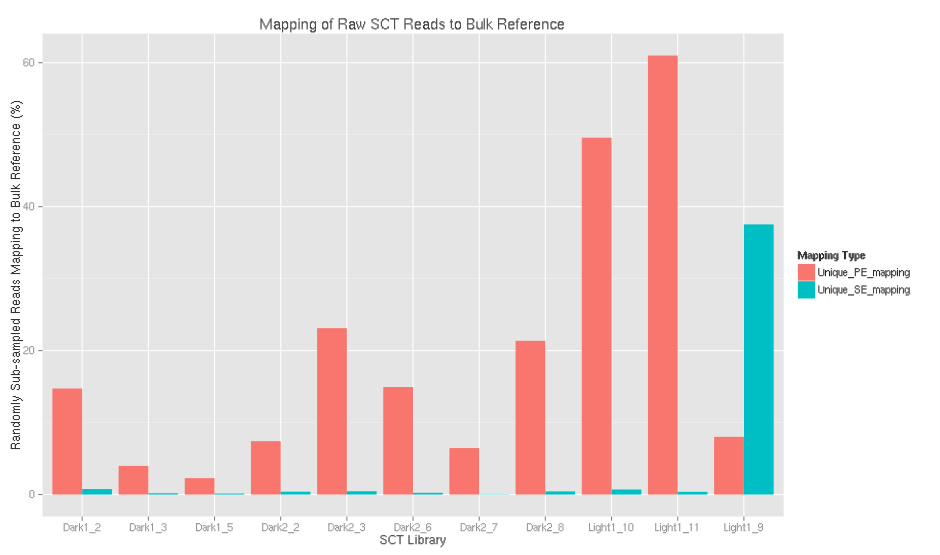
\includegraphics[width=\textwidth]{null_mapping.pdf}
    %plot of parameters random sampling and how they map 
    %null_mapping.svg
    %cutadapt vs trimmomatic plot
    \caption{Null mapping of 5000 randomly sampled PE reads from each SCT library 
                against a reference bulk transcriptome using bowtie2.
                %Of particular interest is the abnormal mapping of Light1\_9 library,
       %     where almost all reads map incongruently with their pair, despite bioanalyser
       %     traces showing fragment size selection with a clear peak at 360-385bp similarly
       % to the other libraries}
            }
    \label{fig:null_mapping}
\end{figure}


\begin{figure}[h]
    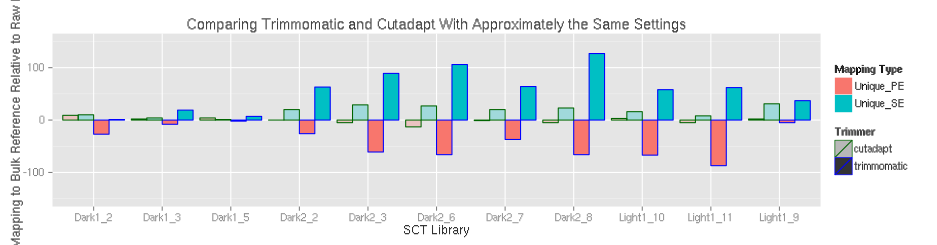
\includegraphics[width=\textwidth]{trimmomatic_vs_cutadapt.pdf}
    %plot of parameters random sampling and how they map 
    %null_mapping.svg
    %cutadapt vs trimmomatic plot
    \caption{Comparison of Trimmomatic and Cutadapt using approximately identical settings:
        specifically minimum length of 60, the entire contents of the Exeter Sequencing Service
        adapter file with respective error rate of 0.03 and Q15 for a simple match and an overall
        error threshold of Q30.

        Interestingly, cutadapt relatively increases the number of PE congruently mapping ends
        relative to untrimmed reads, whereas Trimmomatic generally leads to more PE reads mapping incongruently
        
        However, overall Trimmomatic with these settings has very slightly more paired reads mapping 
        181 vs 180.  

        The other advantages of Trimmomatic outweigh this slight performance deficit
    \label{fig:cvt}
\end{figure}



\subsubsection{Error correction}

Despite numerous indications that error correction is important for improving the accuracy
of genomic and transcriptomic assemblies using Illumina reads (e.g. \citep{Molnar2014,MacManes2015}).
In the case of this dataset error correction appeared to be have a minimal effect with few
reads being corrected and downstream assemblies being largely equivalent (if slightly improved).

Specifically, Bayeshammer as implemented in the Spades genome assembler, even on lightly trimmed
(\(Q>5\)) discarded a maximum \(0.0007\%\) of reads in the 7 selected SCT libraries 
making next to no difference to final assembly.  However, while Bayeshammer is designed for
single cell genomic reads and thus expects uneven coverage as might be found in a transcriptome
it should be noted that it is not specifically designed for RNA-Seq datasets.

Unfortunately, there are still not error correction algorithms directly optimised for scRNA-Seq 
data.  This is potentially due to the relative level of methodological flux still in this 
actively developing area compared to the more established MDA-based single cell genomics methods.

While, there are several available Illumina RNA-Seq error correction tools available 
``SEECER'' was chosen in accordance to the recommendations based on dataset and hardware
heuristics (\(>50M\) reads and the availablility of a high memory system) \citep{Macmanes2015}.


Made very little difference on bulk alone using Seecer
Error 


\subsubsection{GC partitioning}

While the GC partitioning algorithm itself proved very effective 


\subsubsection{Assembly}


%There are \(4^{100}\) possible \(100bp\) reads
%therefore if we randomly sampled from this
%uniformly 
%\(\frac{4.68*10^{5}}{4^{100}}\)





46,819,1  44 characters

reads:


16,054,289,700

NC64A
Input     : 16,054,289,700
Mapped   :    662905 ( 0.4% of input)

We can calculate the probability of matches given
random reads and a random 46.82Mb of host genome
as a generalisation of the birthday 
problem which asymptotically states
\(p\equivalent 1 - exp(-n\frac{n-1}{2d})\)
where \(d = 4^{100}\) i.e. the number of possible
\(100bp\) 4-character reads and \(n =\) 





\begin{table}[h]
\begin{tabular}{|l|rrrrrrrl}
\hline
\multicolumn{1}{|c|}{Assembly} & \multicolumn{1}{c|}{Raw Reads (paired)} & \multicolumn{1}{c|}{\begin{tabular}[c]{@{}c@{}}Trimmed Reads \\ (assuming all paired)\end{tabular}} & \multicolumn{1}{c|}{Assembled Contigs} & \multicolumn{1}{c|}{Assembled "Genes"} & \multicolumn{1}{c|}{"Gene" N50} & \multicolumn{1}{c|}{"Gene" Mean Length} & \multicolumn{1}{c|}{"Gene" Total Assembled Bases} & \multicolumn{1}{c|}{GC\%} \\ \hline
Kodama Trinity                 & 232.3M                                  & 218.5M                                                                                              & 68,175                                 & 40,805                                 & 904                             & 1,832                                   & 36.9M                                             & \multicolumn{1}{c}{?}     \\ \cline{1-1}
SCT Q30                        & 126.9M                                  & 93.2M                                                                                               & 99,784                                 & 88,573                                 & 475                             & 451                                     & 40.0M                                             & 48.67                     \\ \cline{1-1}
SCT Q30 + Bulk                 & 179.4M                                  & 145.6M                                                                                              & 127,508                                & 103,506                                & 646                             & 564                                     & 58.2M                                             & 40.30                     \\ \cline{1-1}
SCT Q5                         & 126.9M                                  & 108.2M                                                                                              & 112,182                                & 99,441                                 & 465                             & 447                                     & 44.5M                                             & 49.42                     \\ \cline{1-1}
SCT Q5 + Bulk                  & 179.4M                                  & 160.6M                                                                                              & 139,226                                & 113,685                                & 615                             & 549                                     & 62.5M                                             & 41.28                     \\ \cline{1-1}
Bulk                           & 52.4M                                   & 52.4M                                                                                               & 43,261                                 & 30,706                                 & 1264                            & 861                                     & 26.5M                                             & 29.61                     \\ \cline{1-1}
\end{tabular}
\end{table}



\subsubsection{Saturation}

\subsection{Binning}

%Fortunately, to this end, the only other published 2nd generation sequencing analysis of \textit{P. bursaria} and a green algal,
%endosymbiont: Kodama \textit{et. al.} 2014 \citep{Kodama2014} partially addressed this issue.  This analysis investigated 
%the differential global metatranscriptome profile of \textit{P. bursaria} Yad1g strain with and without its \textit{Chlorella variabilis} 1N endosymbiont 
%\citep{Kodama2014}.   While, this is a different strain of both host and endosymbiont to the CCAP1660/12 strains (\textit{P. bursaria} and \textit{Micractinium reisseri}) 
%used in this thesis it offers a potential avenue to investigate these other components.
%An attempt was made to replicate this work using the CCAP1660/12 strains, unfortunately, elimination of the endosymbionts without death of the host
%didn't prove possible in these strains.  Despite using 
%
%(despite earlier publications to the contrary) by either maintaining the culture in the dark \citep{Siegel1960} (although some studies have thrown doubt on
%        how effective this method is at completely elimiating the photobiont \citep{Tanaka2002}) or treatment with various titrations of herbicides 
%            (e.g. paraquat \citep{Hosoya1995a}) or the protein synthesis inhibitor cyclohexamide \citep{weis1984effect}).\footnote{
%        There are naturally aposymbiotic strains of \textit{Paramecium bursaria} \citep{Tonooka2002a}}



\section{Conclusion}
In conclusion,

Library filtering is key with single cell possibly due to the increased inefficiency of poly-A selection

GC partitioning doesn't work - splits up contigs

Trimming and error correction makes little difference on unsaturated complex single cell 

Arboretum offers a useful way to accurately classify transcripts into likely origins 



